\section{How Do Interpretations Help?}
\label{sec:help}

This section explores how model interpretations help to guide adversarial
authors. We analyze the question edit log, which reflects how authors
modify questions given a model interpretation.

A direct edit of the highlighted words often creates an
adversarial example (e.g., Figure~\ref{fig:success}).
Figure~\ref{fig:edit_example_1} shows a more intricate example. The
left plot shows the \emph{Question Length}, as well as the
position where the model is first correct (\textit{Buzzing Position},
lower is better). We show two adversarial edits. In the first
(\textbf{1}), the author removes the first sentence of the question,
which makes the question \emph{easier} for the model (buzz position
decreases). The author counteracts this in the second edit (\textbf{2}),
where they use the interpretation to craft a targeted modification which
breaks the \abr{ir} model.

However, models are not always this brittle. In
Figure~\ref{fig:failure} (Appendix~\ref{sec:failed}), the interpretation fails to aid an
adversarial attack against the \abr{rnn} model. At each step, the
author uses the highlighted words as a guide to edit targeted portions
of the question yet fails to trick the model. The author gives up and
submits their relatively non-adversarial question.

\begin{figure}[h]
\centering
\tikz\node[draw=black!40!green,inner sep=1pt,line width=0.3mm,rounded corners=0.1cm]{
\begin{tabular}{p{0.46\textwidth}}
One of these concepts $\ldots$ a \textbf{Hyperbola} is a type of, for ten
points, what shapes made by passing a \textbf{plane} through a namesake solid, \\
\mybox{gitred}{\sout{that also includes the \textbf{ellipse}, \textbf{parabola}?}} \\
\mybox{gitgreen}{whose area is given by one-third Pi r squared} \mybox{gitgreen}{times height?} \\
\emph{Prediction}: \underline{Conic Section} (\Checkmark) $\to$ \underline{Sphere} (\xmark)
\end{tabular}
};
\caption{The interpretation successfully aids an attack
  against the \abr{ir} system. The author removes the phrase containing the words
  ``ellipse'' and ``parabola'', which are highlighted in the interface (shown
  in bold). In its place, they add a phrase which the model associates with the
  answer \underline{sphere}.}
\label{fig:success} 
\end{figure}

\subsection{Interviews With Adversarial Authors}

We also interview the adversarial authors who attended our live events. Multiple authors agree that identifying oft-repeated ``stock'' clues was the interface's most useful feature. As one author explained, ``There were clues which I did not think were stock clues but were later revealed to be''. In particular, the author's question about the \underline{Congress of Vienna} used a clue about ``Krak\'ow becoming a free city'', which the model immediately recognized.

Another interviewee was Jordan Brownstein,\footnote{\url{https://www.qbwiki.com/wiki/Jordan_Brownstein}} a national \qb{} champion and one of the best active players, who felt that computer opponents were better at questions that contained direct references to battles or poetry. He also explained how the different writing styles used by each \qb{} author increases the difficulty of questions for computers. The interface's evidence panel allows authors to read existing clues which encourages these unique stylistic choices.

\begin{figure*}
\centering
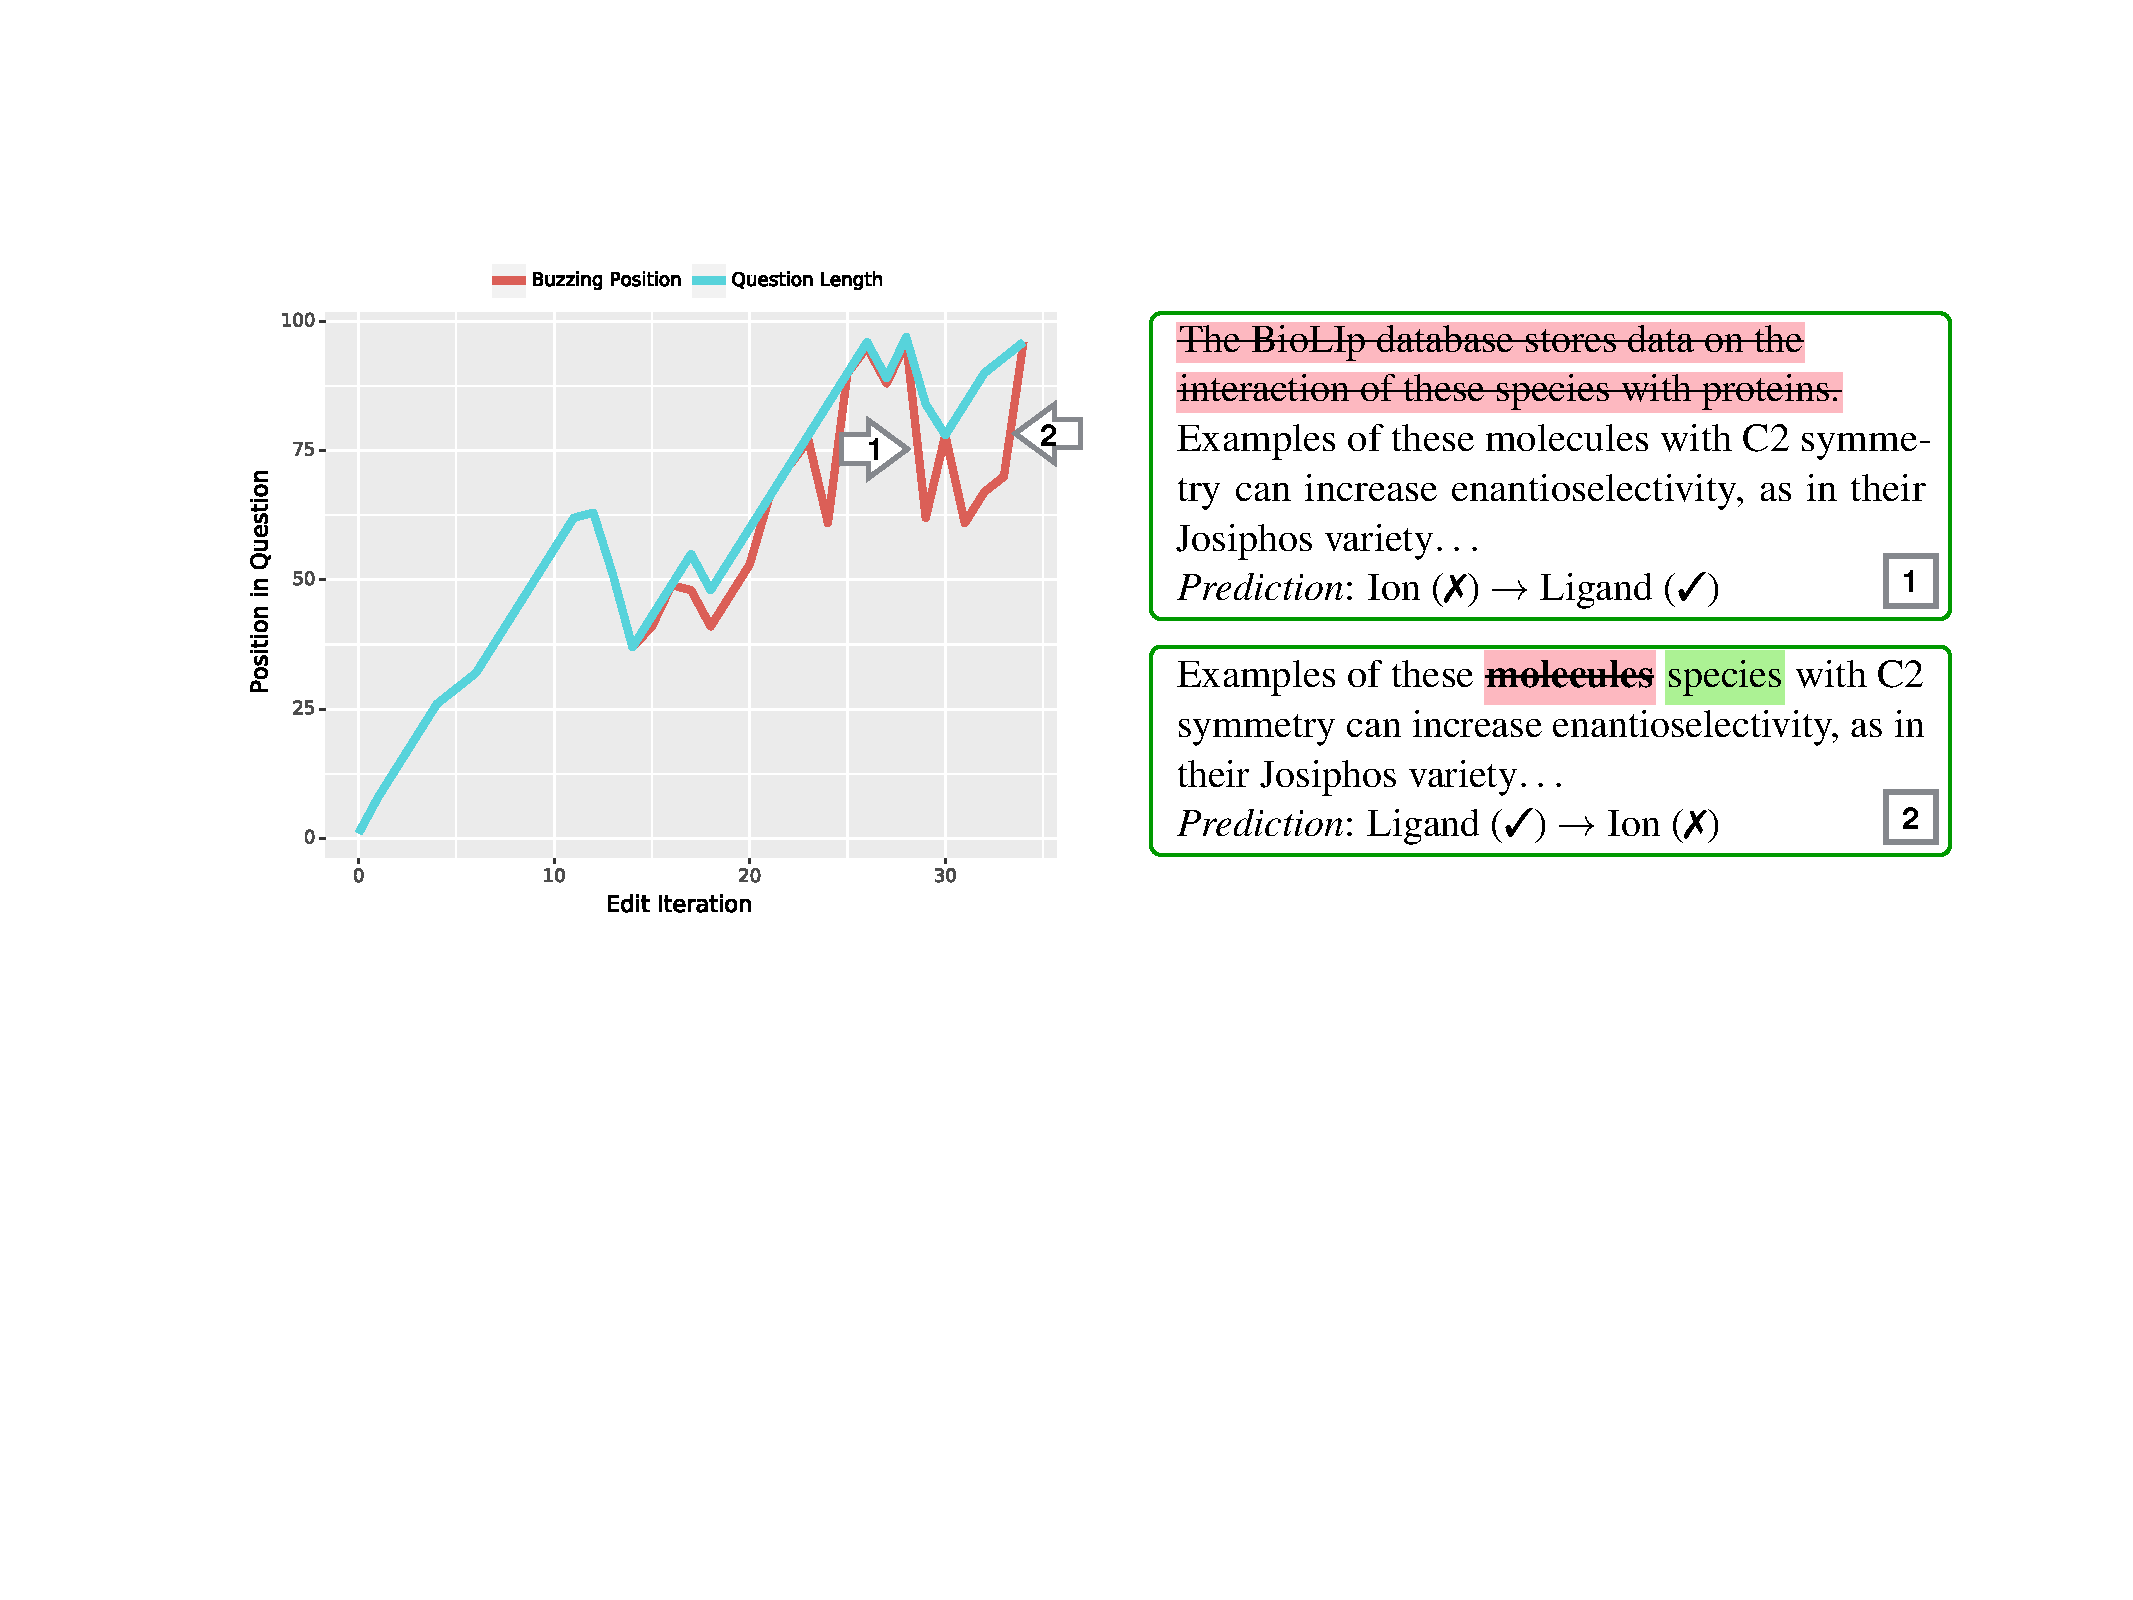
\includegraphics[width=\textwidth]{edit_example_1}
\caption{The \emph{Question Length} and the
  position where the model is first correct (\textit{Buzzing
    Position}, lower is better) are shown as a question is written. In (\textbf{1}), the author makes a
  mistake by removing a sentence that makes the question easier for the \abr{ir} model. In
  (\textbf{2}), the author uses the interpretation, replacing the
  highlighted word (shown in bold) ``molecules'' with ``species'' to trick
  the \abr{rnn} model.}
\label{fig:edit_example_1}
\end{figure*}